\documentclass[border=5pt]{standalone}
\usepackage{tikz}
\usetikzlibrary{arrows.meta, positioning}
\usepackage{xcolor}

\definecolor{Garnet}{HTML}{73000A}
\definecolor{Atlantic}{HTML}{466A9F}
\definecolor{Horseshoe}{HTML}{65780B}
\definecolor{TenBlack}{HTML}{ECECEC}

\begin{document}
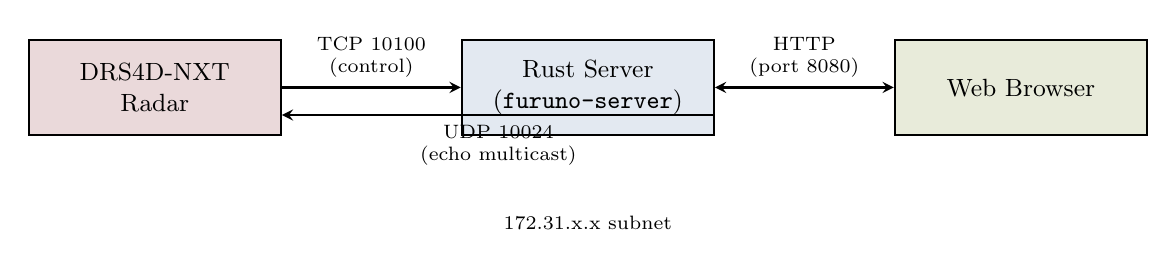
\begin{tikzpicture}[
  box/.style={draw, thick, minimum width=3.2cm, minimum height=1.2cm, align=center, font=\small},
  lbl/.style={font=\scriptsize, align=center},
  >=stealth
]
  \node[box, fill=Garnet!15] (radar) at (0,0) {DRS4D-NXT\\Radar};
  \node[box, fill=Atlantic!15] (server) at (5.5,0) {Rust Server\\(\texttt{furuno-server})};
  \node[box, fill=Horseshoe!15] (browser) at (11,0) {Web Browser};

  \draw[->, thick] (radar.east) -- node[above, lbl] {TCP 10100\\(control)} (server.west);
  \draw[<-, thick] (radar.east) ++ (0,-0.35) -- node[below, lbl] {UDP 10024\\(echo multicast)} ++ (5.5,0);
  \draw[<->, thick] (server.east) -- node[above, lbl] {HTTP\\(port 8080)} (browser.west);

  \node[lbl, below=0.9cm of server] {172.31.x.x subnet};
\end{tikzpicture}
\end{document}
